\section{State of research}
\label{sec:state_of_research}
This chapter provides an overview of related researches in the field of software evolution analysis. The related work addresses how information of version control and issue tracking systems can be investigated by using specific analyzation methods.

%Populating a Release History Database from Version Control and Bug Tracking Systems:
\subsection{Release History Database}
The anlayzation method by Fischer et al. \cite{fischer2003populating} uses a release history database (RHDB) to research the software evolution of development projects. The RHDB is populated with version data of version control systems and bug tracking data of bug repositories. Once the RHDB is populated, it is possible to execute simple queries to the structured data. Those queries produce specific views that enable an accurate reasoning of evolutionary aspects of software evolution \cite{fischer2003populating}.
Fischer et al. tested their approach on the large Open Source project Mozilla Firefox \cite{mozilla}. In this project, the analyzed version control data is managed with the CVS \cite{cvs} system, while the bug data is stored in the Bugzilla \cite{bugzilla} issue tracking system. 

To populate the RHDB, Fisher et al. extracted the data of both systems and imported it into the database. This was implemented by different Shell and Perl scripts that process the data and inserted it into the RHDB. The entity relationship (ER) model of the RHDB is shown in figure \ref{fig:rhdber} \cite{fischer2003populating}. There are according tables for data of the CVS version control system and the issue tracking system. For the CVS repository information, the important tables are \textbf{cvsitem}, \textbf{cvsitemlog} and \textbf{cvsauthor}. Therefore, the CVS artifact attributes are stored in the \textbf{cvsitem} table. Modification report data is stored in \textbf{cvsitemlog} and the author name of every CVS artifact is stored in the \textbf{cvsauthor} table. However, the bug report artifacts are stored in the \textbf{bugreport} table, whereas the description of a bug is stored in the \textbf{bugreportdesc} table. The connection between \textbf{cvsitemlog} and \textbf{bugreport} would be a n:n relation, hence it is resolved by a \textbf{cvsitemlogbugreport} table.

\begin{figure*}[t]
	\centering
	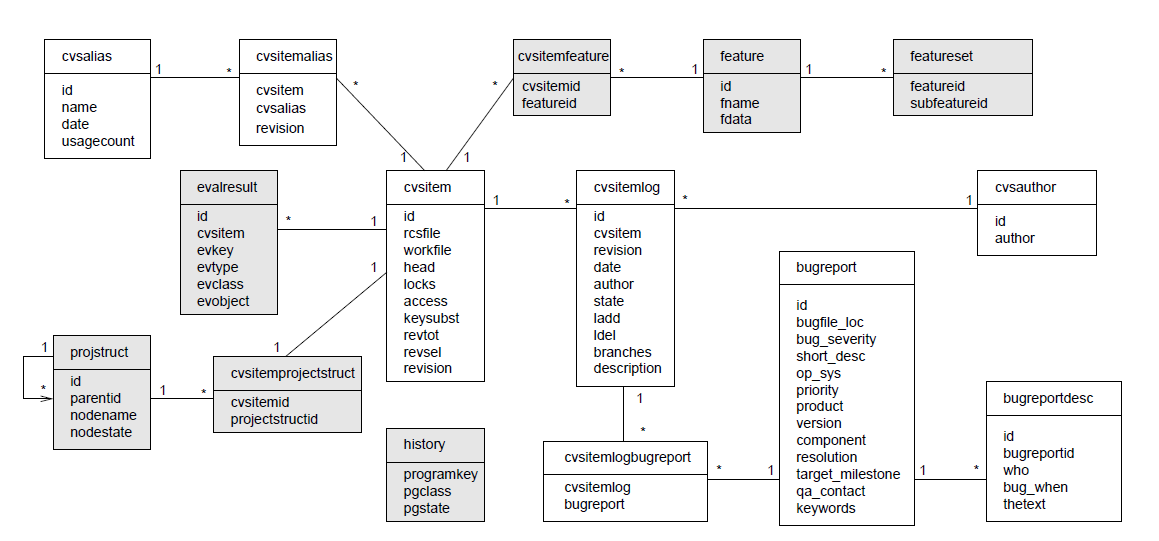
\includegraphics[width=0.8\textwidth]{images/rhdb_er}
	\caption{RHDB ER-Model \cite{fischer2003populating}}
	\label{fig:rhdber}
\end{figure*}

With this RHDB ER-Model it is possible to execute SQL-queries that can present a view on software evolution of the project. A sample query to list all bug reports for \textit{nsNSSDialogs.cpp}, presented by Fischer et al. is e.g. \cite{fischer2003populating}:

\begin{verbatim}
SELECT
	b.bugreport, r.bug_severity, r.short_desc
FROM
	cvsitem i, cvsitemlog l,
	cvsitemlogbugreport b, bugreport r
WHERE 	
	i.id = l.cvsitem
	AND l.id = b.cvsitemlog
	AND b.bugreport = r.id
	AND i.rcsfile REGEXP 'nsNSSDialogs.cpp';
	
\end{verbatim}

The application of the method on the Mozilla project stated that it was possible to link bug reports with version control data in an effective way \cite{fischer2003populating}. 

%Wie hat sich die Wissenschaft bis jetzt entwickelt?
%Wer hat welche Voraussetzungen geschaffen?
%Welche vergleichbaren Ergebnisse gibt es bisher?
%Welche Fragen sind noch offen?
%Warum reicht das bisher Getane noch nicht?
%Soll eine bestimmte These widerlegt oder bestätigt werden?
%Welche sind die wichtigen Veröffentlichungen? Was sagen sie zum Thema?